\appendix
\section{Abschwächung des Lasers}
\label{sec:laser}
In der folgenden Rechnung wird berechnet, wie stark das Laserlicht abgeschwächt
werden muss, damit mit \SI{99,9}{\percent}iger Wahrscheinlichkeit nur ein
einziges Photon pro Puls an der Photodiode ankommt. Dafür wird verwendet, dass
die Photonenzahl beim Laser einer Poisson-Statistik unterliegt. Zunächst muss
berechnet werden, wie viele Photonen sich in einem Puls befinden (Photonenzahl
$N_P$), und anschließend kann bestimmt werden, um welchen Faktor die Intensität
verringert werden muss, um die genannte Wahrscheinlichkeit zu erreichen, nur ein
einziges Photon zu detektieren.
\begin{eqnarray}
E_{\mathrm{Puls}} &=& \SI{50}{mW}\cdot\SI{10}{ns} = \SI{50e-12}{J}\\
E_{\mathrm{Photon}} &=& hν = h\frac{c}{λ}\\
N_P &=& \frac{E_{\mathrm{Puls}}}{E_{\mathrm{Puls}}} = \SI{1,6e8}{}
\end{eqnarray}
Dies entspricht dem Erwartungswert λ der Photonenanzahl.
\begin{eqnarray}
P_λ(X=k) &=& \frac{λ^k}{k!}\mathrm{e}^{-λ}\\
\rightarrow P_{kλ}(1) &=& kλ\mathrm{e}^{-kλ} = \SI{0.999}{}
\end{eqnarray}
Hierbei ist $k$ eine Konstante, die beschreibt, welcher Anteil des Lichts die
Filter passieren soll. Diese Gleichung kann numerisch gelöst werden, wobei sich
hier das folgende für $k$ ergibt:
\begin{equation}
k = \SI{1.2e6}{}
\end{equation}
Wenn also die Filter so gewählt werden, dass die Intensität um einen Faktor von
ca. $10^6$ verringert wird, kann man davon ausgehen, dass nur ein Photon eines
Pulses den Detektor erreicht.

\section{Wahl der Polarisation}
\label{sec:zirkular}
Text.

\onecolumn
\section{Messprotokoll}
\label{sec:protokoll}
\begin{figure}[!ht]
        \centering
        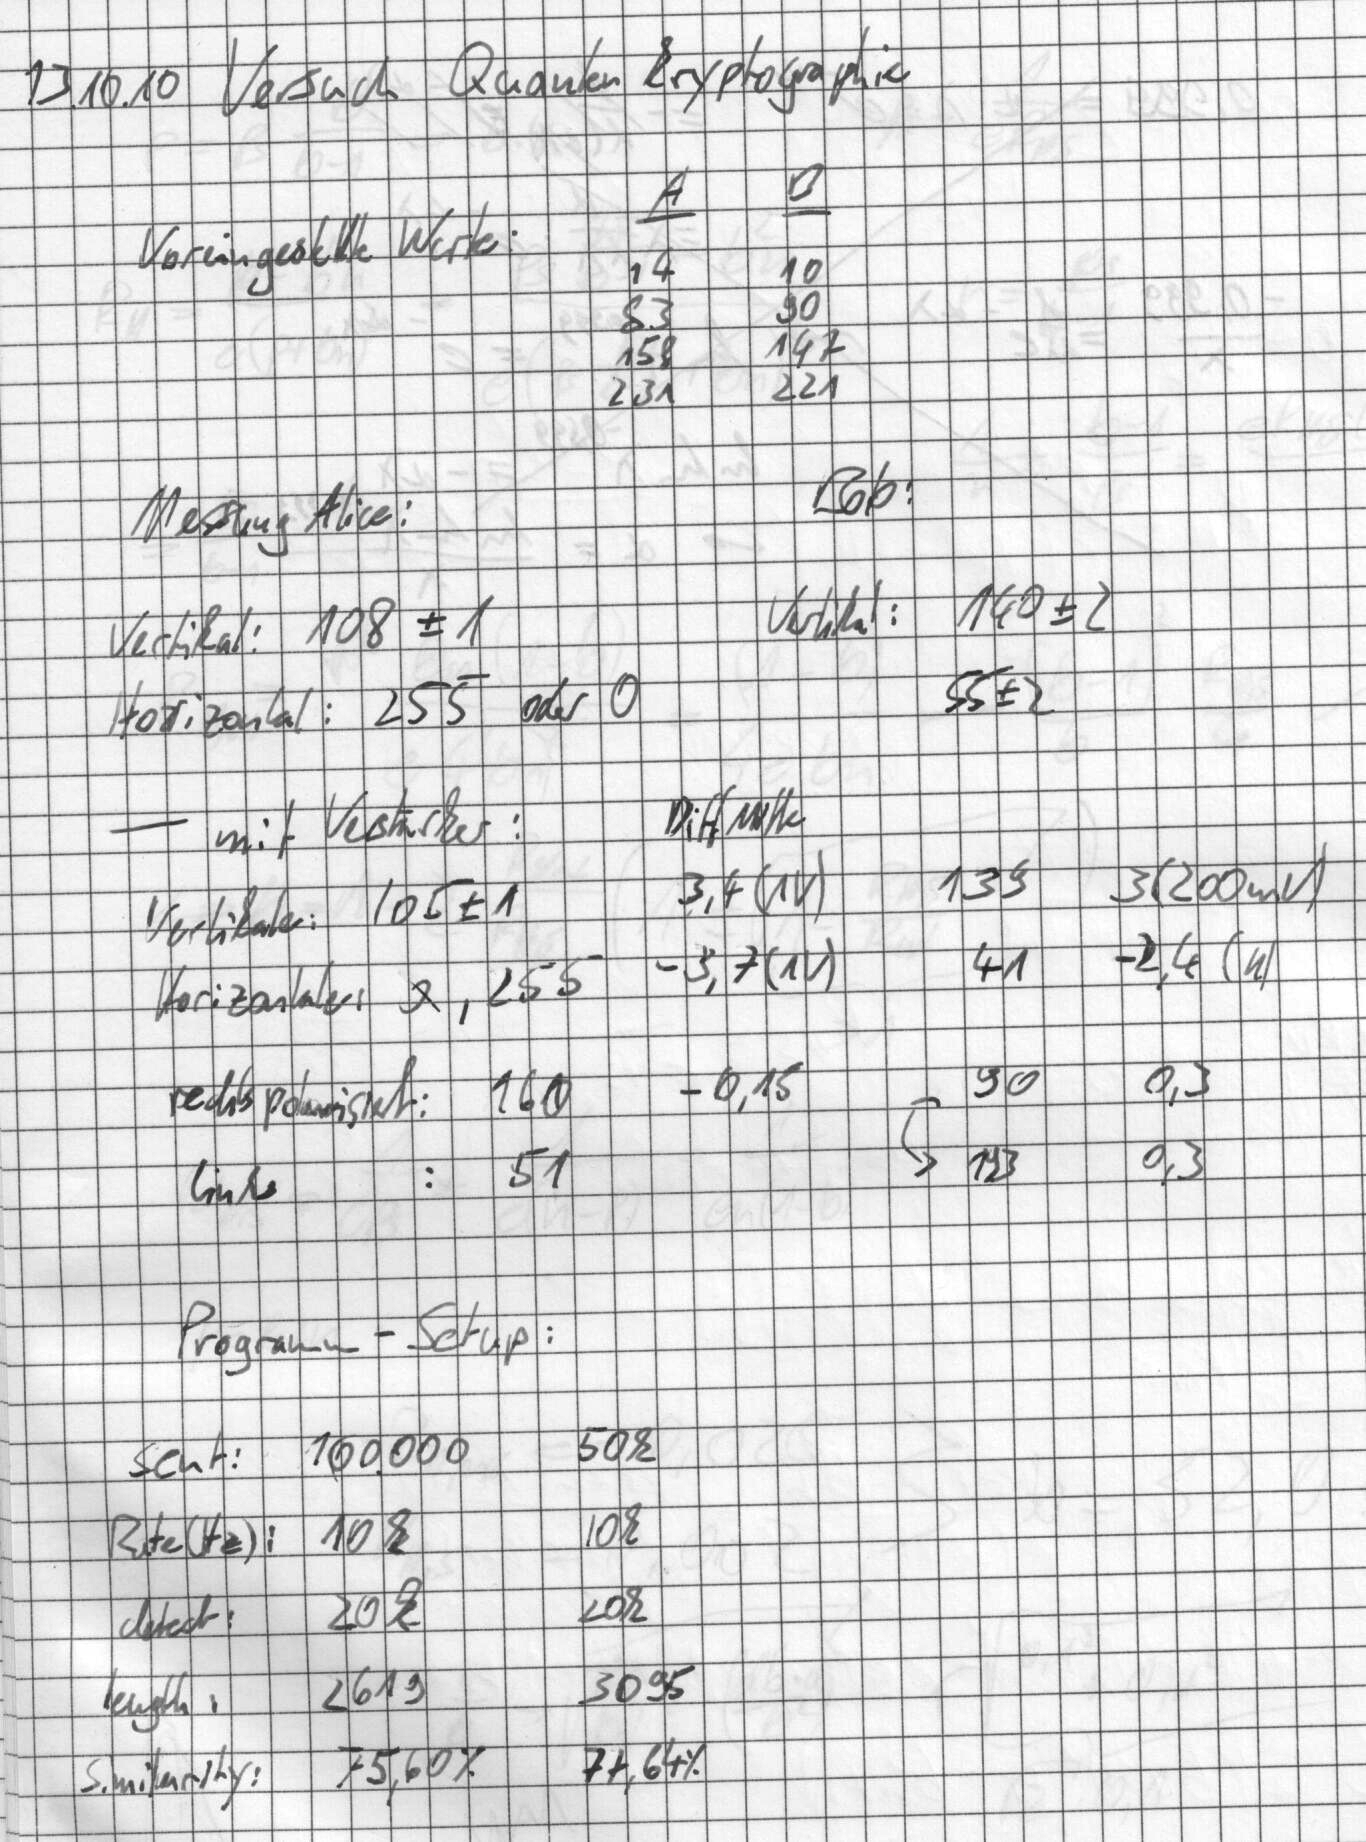
\includegraphics[page=1,width=.88\textwidth,keepaspectratio]{../data/messprotokoll}
%         \caption{Messprotokoll}
        \label{fig:protokoll}
\end{figure}